\documentclass[journal]{IEEEtran}

\ifCLASSINFOpdf
\else
   \usepackage[dvips]{graphicx}
\fi
\usepackage{url}

\hyphenation{op-tical net-works semi-conduc-tor}

\usepackage{graphicx}

% Macro to get code font
\def\code#1{\texttt{#1}}


\begin{document}

\title{AMATH 582 Homework 1: An Ultrasound Problem}

\author{Eric A. Silk
\thanks{Eric Silk is a Masters Student in Applied Mathematics at the University of Washington,
		and a Research Engineer for Schweitzer Engineering Laboratories, Pullman, WA 99163 (email: esilk16@uw.edu, eric.silk@ericsilk.com)}
}

\markboth{Homework Submission for AMATH 582: Computational Methods for Data Analysis, January 2020}
{Shell \MakeLowercase{\textit{et al.}}: Bare Demo of IEEEtran.cls for IEEE Journals}
\maketitle

\begin{abstract}
This paper serves to describe the process by which a noisy ultrasound can be cleaned and analyzed to determine the path of an foreign object within the intestines of a dog. Through the use statistical methods, Fast Fourier Transforms, spectrum averaging, and Gaussian filtering, highly noisy data can be resolved into a clear trajectory.
\end{abstract}

\begin{IEEEkeywords}
Filter, Fourier, Gaussian, Histogram, Spectrum, Ultrasound
\end{IEEEkeywords}


\IEEEpeerreviewmaketitle



\section{Introduction}

\IEEEPARstart{I}{n} the example proposed by Dr. Kutz, a dog has swallowed a marble and it is moving through its intestines. 20 ultrasound measurements were taken sequentially in time, producing three-dimensional matrices of the local magnitudes. Unfortunately, they are highly noisy. In order to determine the trajectory of the marble, filtering must be employed to remove the noise.

\section{Theoretical Background}
Ultrasounds produce spatial data, indicating the intensity of the reflection of an acoustic wave off of a surface at some distance. Objects produce reflections at characteristic frequencies, even as their physical position may change. This fact can be exploited to isolate a given object within a noisy environment and determine its trajectory through multiple measurements.

\subsection{Fourier Transforms}
Converting a temporal or spatial problem into the frequency domain can be achieved with a Fourier transform (Equation \ref{fourier})

\begin{equation}
\label{fourier}
\hat{f}(\omega)=\int_{-\infty}^{\infty}f(x)e^{-2 \pi jx \omega}dx
\end{equation}

This assumes a given section of data is periodic and fully contained within the range of $-\pi$ to $\pi$. This requires the results be scaled appropriately (Equation \ref{scaling}).

\begin{equation}
\label{scaling}
\omega_{scaled}=\frac{\pi}{L}\omega_{nominal}
\end{equation}

\noindent where the signal exists between in the region $[-L:L)$.

Given that processing is occurring on a computer, the Discrete Fourier Transform (Equation \ref{dft}), or ``DFT'' is used -- in particular, the Fast Fourier Transform (hereafter ``FFT'').

\begin{equation}
\label{dft}
X_{k}=\sum_{n=0}^{N-1}x_{n}e^{-\frac{j2\pi}{N}kn}
\end{equation}

The FFT works by recursively decomposing the transform into 2 smaller transforms until a prime length is reached (ideally 1) along some branch of the recursion, then shifting the results in a "butterfly" fashion. For this reason, FFT's of size $2^n$ are fastest, but any vector with small prime factors will perform reasonably quickly.

\subsection{Noise}
Here, noise is defined as the signal produced by a stochastic, stationary phenomena unrelated the primary signal of interest. These may include the random fluctuations of electrons within the measuring apparatus, movement of fluids within the dog's body, or the process of discretizing analog measurements.

Noise is often characterized by its distribution within the frequency spectrum. For instance, white noise has equal intensities across the whole spectrum, producing a signal with a finite variance and zero mean. Thus, while a single measurement of white noise may produce a fairly energetic spectrum, averaging multiple measurements will tend towards a zero energy spectrum.

Utilizing these pieces of information, the 20 provided measurements can be averaged to force any white noise present towards zero, while preserving the frequency components of the object of interest. Once these frequencies are determined, a filter can be applied to remove noise in individual measurements. Doing so will allow the trajectory of the marble to be determined.

\subsection{Gaussian Filter}
Gaussian filters are commonly used in image processing to reduce noise and smooth data, and are fairly straightforward to implement. As such, it was deemed an appropriate choice for the problem of filtering the data. They can be created in arbitrary dimensions, including 1D (Equation \ref{gauss1D}) and 3D (Equation \ref{gauss3D})

\begin{equation}
\label{gauss1D}
G(x)=\frac{1}{\sqrt{2\pi\sigma^2}}e^{-\frac{(x-x_{\omega})^2}{2\sigma^2}}
\end{equation}

\begin{equation}
\label{gauss3D}
G(x,y,z)=\frac{1}{\sqrt{2\pi\sigma^2}}e^{-\frac{(x-x_{\omega})^2+(y-y_{\omega})^2+(z-z_{\omega})^2}{2\sigma^2}}
\end{equation}

$x_{\omega}$, $y_{\omega}$, and $z_{\omega}$ are the frequencies to shift the center of the kernel to. These equations assume the same variance in all dimensions.

\section{Algorithm Implementation and Development}
The first portion of work involved exploring the \code{isosurface} plots of each sample, which proved largely fruitless (Fig. \ref{spatial_isosurface}). The data is highly noisy, and attempts at increasing the threshold of the \code{isosurface} plot were ineffective in isolating the trajectory of the marble. Next, \code{fftn} was used to take a multidimensional FFT of each sample. The absolute value of the results of these were also plotted via \code{isosurface} (taking care to \code{fftshift} the data) with little success -- the Fourier transform of noisy data produces a noisy spectrum. An example can be seen in Fig. \ref{freq_isosurface}. 

\begin{figure}
	\centerline{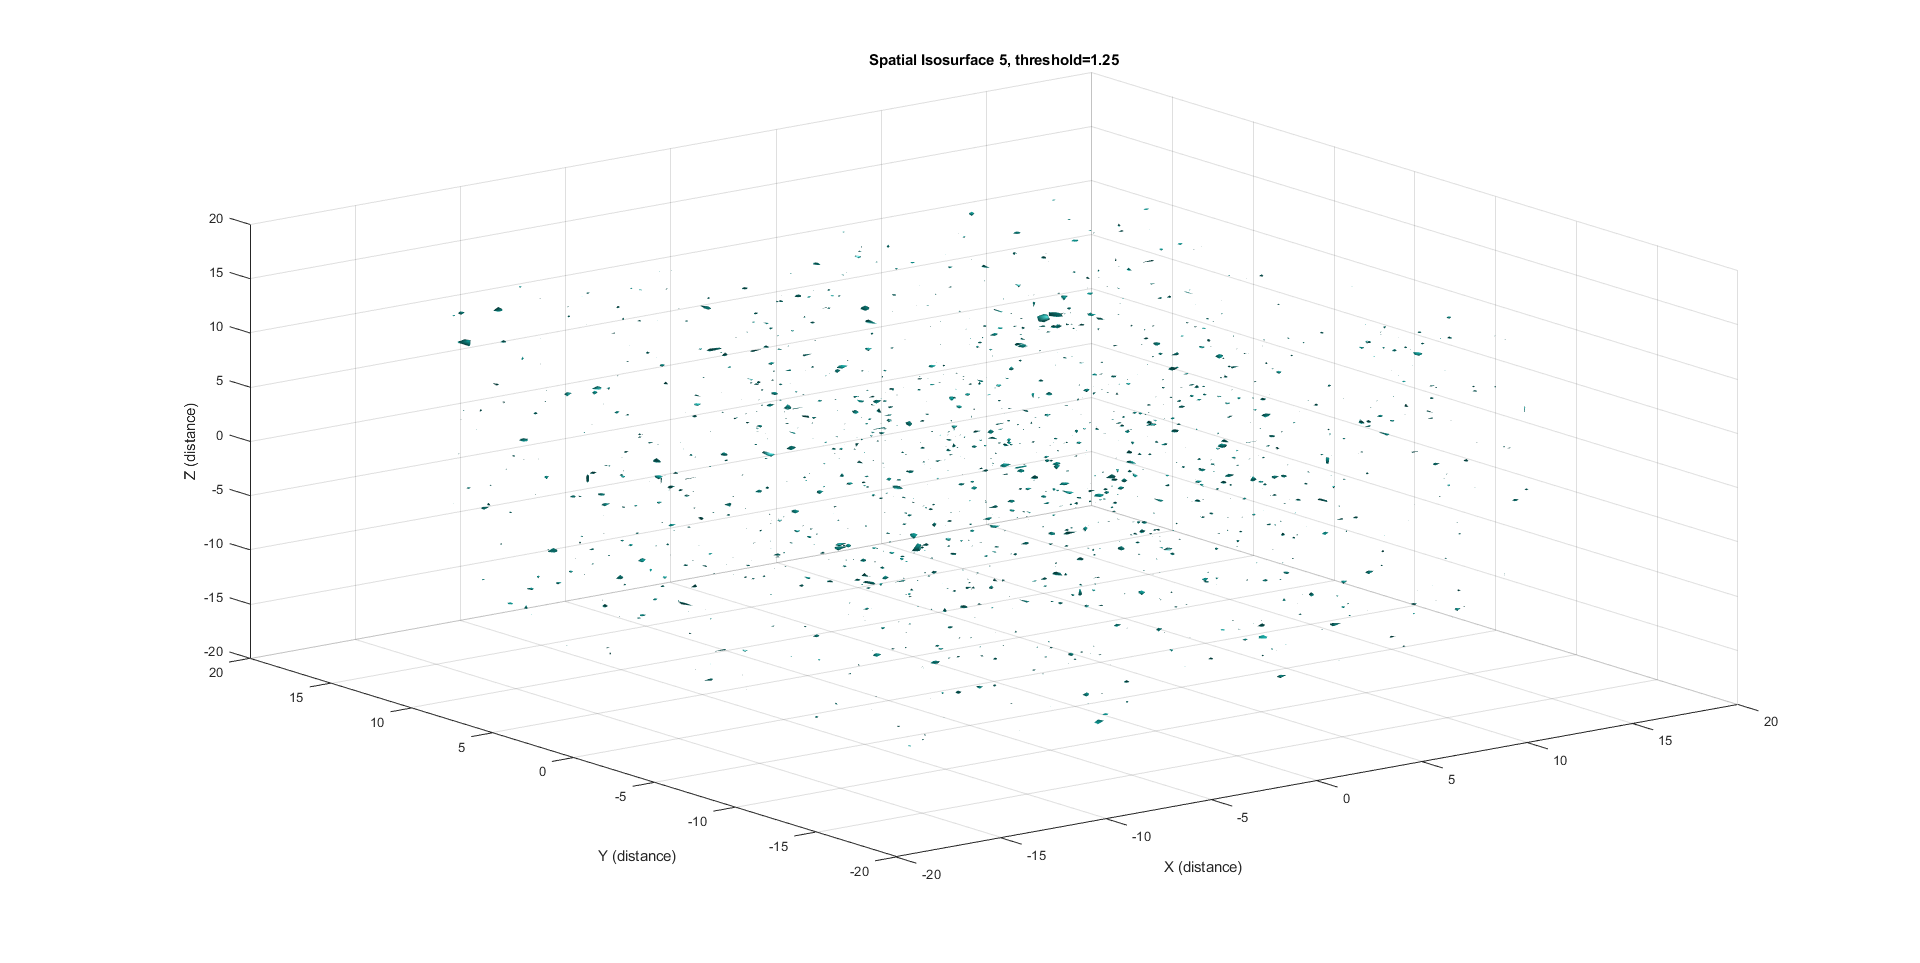
\includegraphics[width=\columnwidth]{spatial_isosurface.png}}
	\caption{Thresholded spatial isosurface, showing the clearly noisy data.}\label{spatial_isosurface}
\end{figure}

\begin{figure}
	\centerline{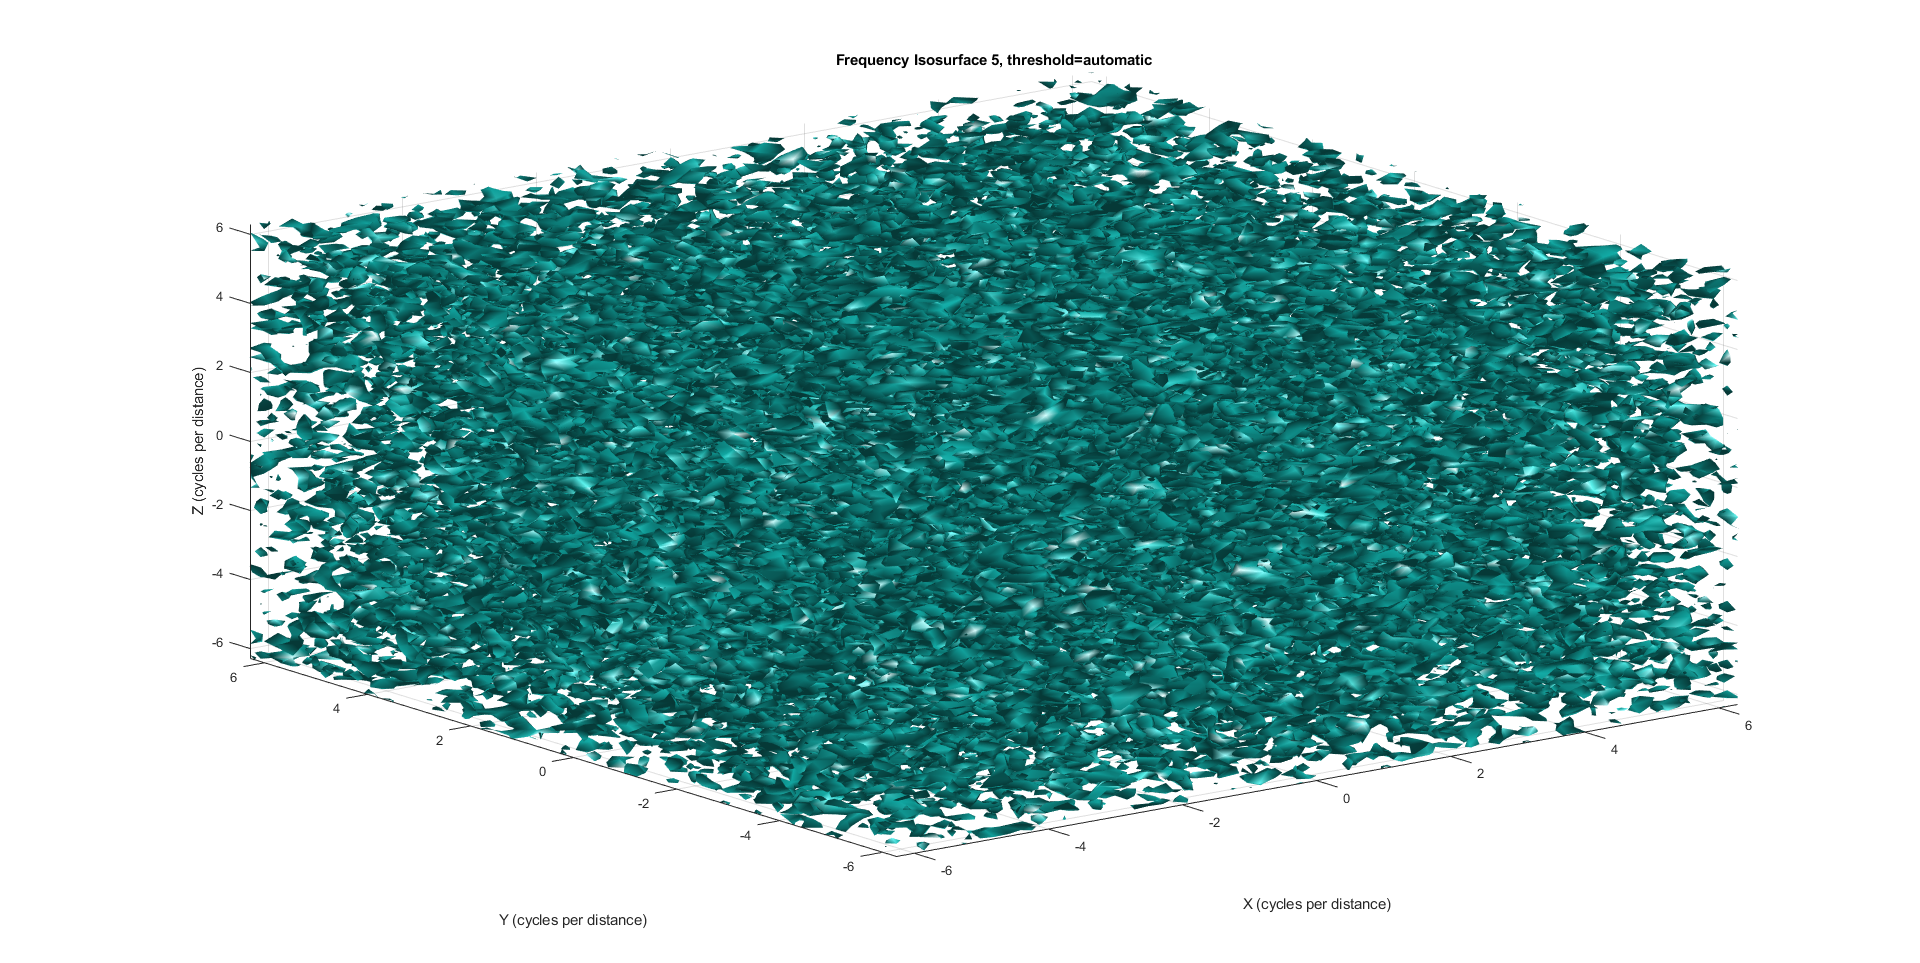
\includegraphics[width=\columnwidth]{freq_isosurface.png}}
	\caption{Thresholded frequency isosurface, showing the clearly noisy data.}\label{freq_isosurface}
\end{figure}


A loop was used to sum each sample's spectrum together, before dividing by the number of samples to average the spectrums. This was done to take advantage of the previously mentioned zero mean of noise. In addition, while looping, a histogram of the absolute value of the spectrum was plotted (Fig. \ref{freq_hists}). Finally, a histogram of the resulting averaged spectrum was plotted to visually verify the shift in the spectrum (Fig. \ref{avg_hist}.

\begin{figure}
	\centerline{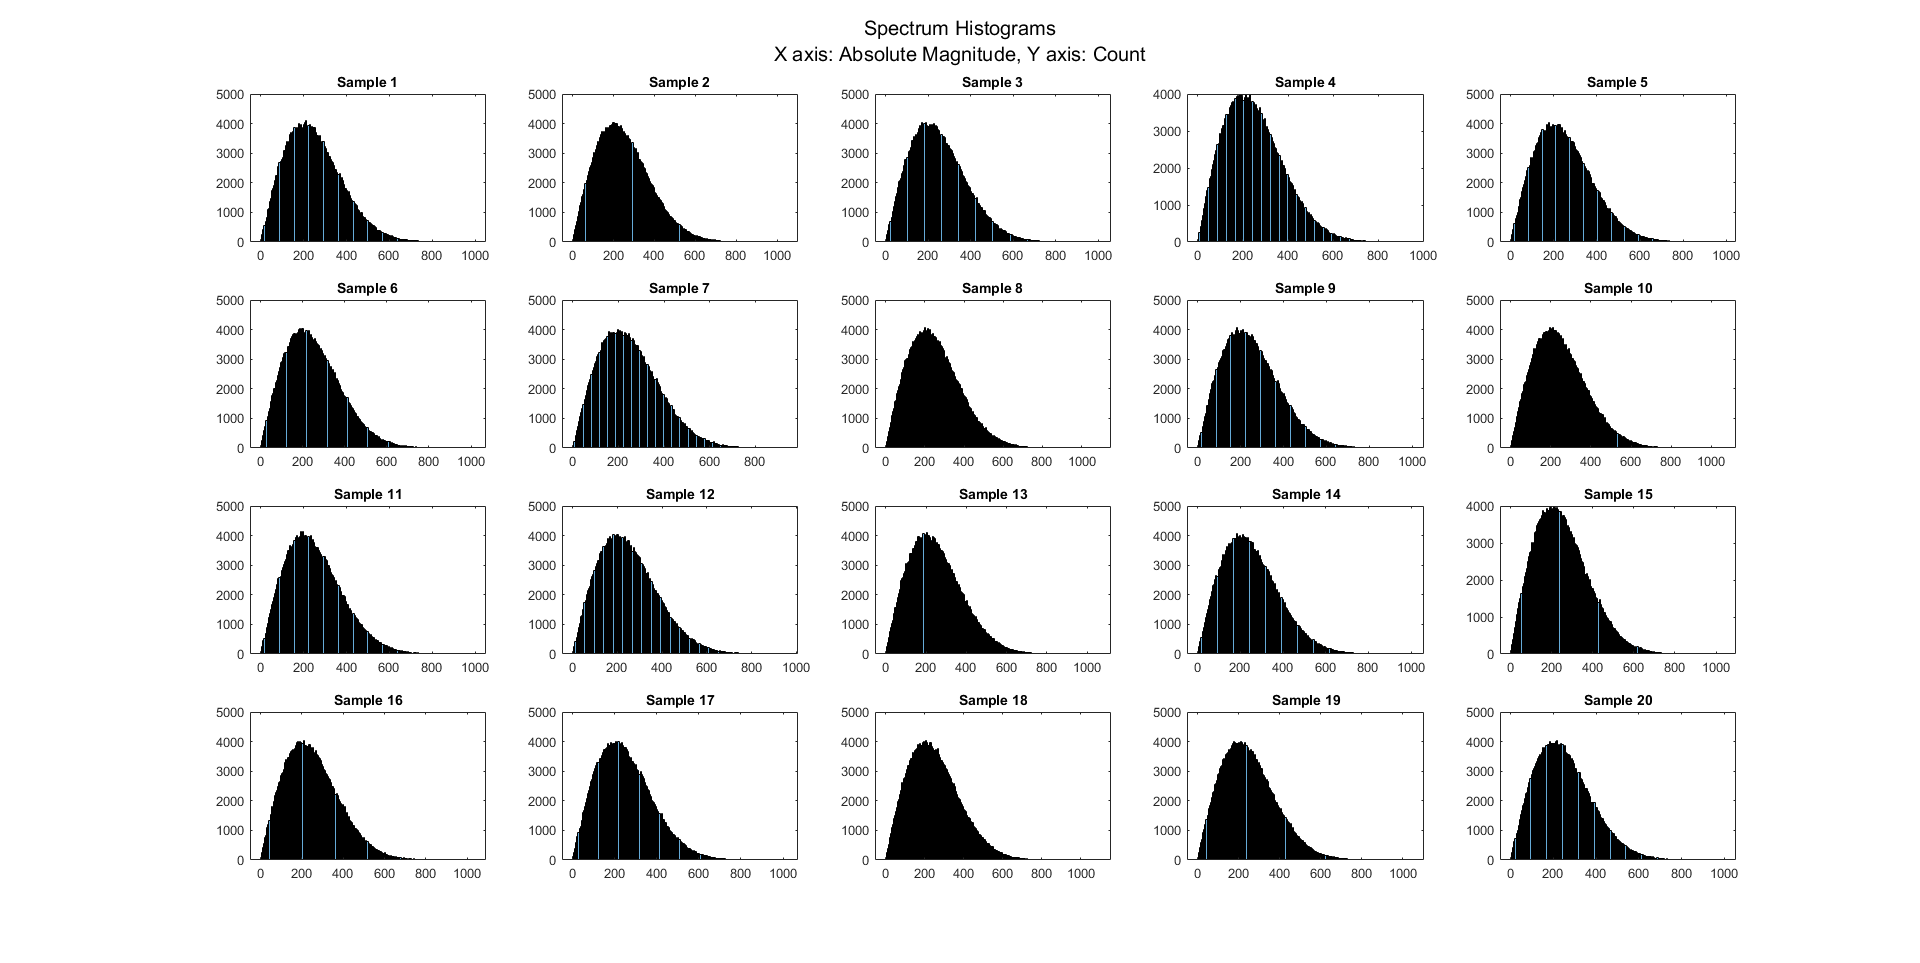
\includegraphics[width=\columnwidth]{spectrum_hists.png}}
	\caption{Histograms of the frequency spectrum for each sample.}\label{freq_hists}
\end{figure}

\begin{figure}
	\centerline{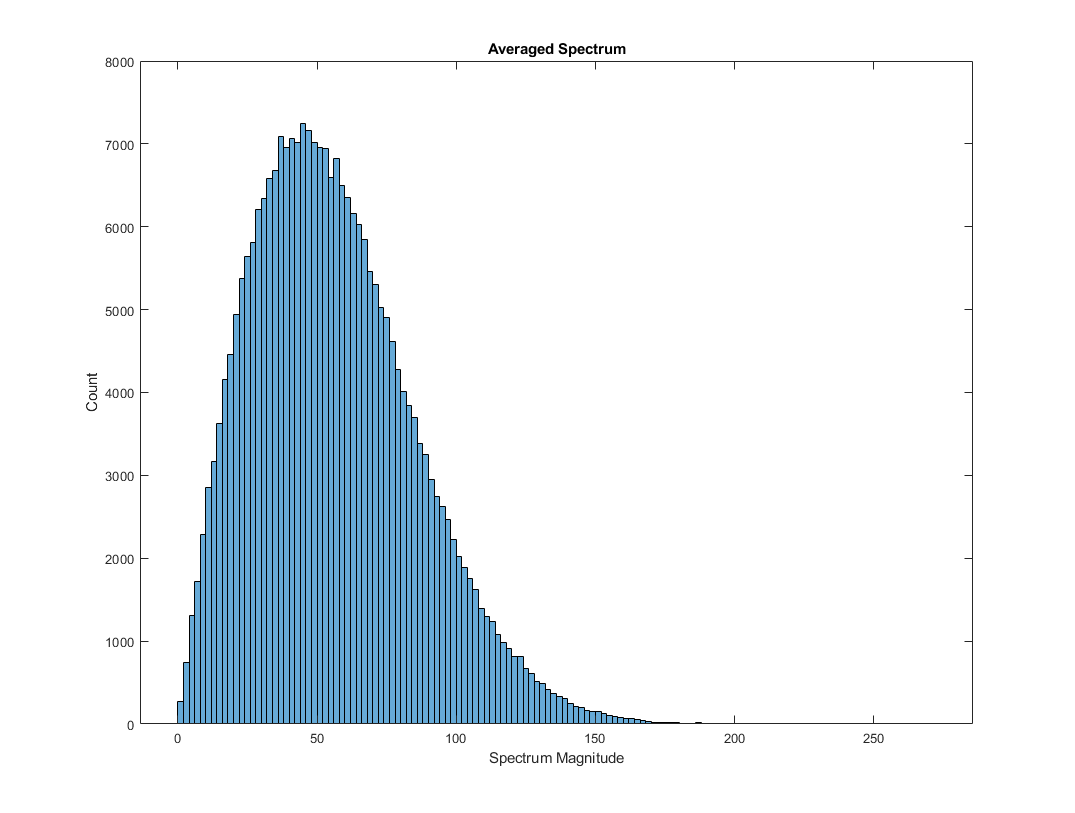
\includegraphics[width=\columnwidth]{averaged_spectrum_hist.png}}
	\caption{Histograms of the frequency spectrum for each sample.}\label{avg_hist}
\end{figure}

This averaged spectrum was then plotted via \code{isosurface}, with increasing thresholds (informed by the distribution of the histogram). A more rigorous, fully automatic method (e.g. threshold on percentile) would be preferred in a production environment. From this a trend to exclude more and more noise can be seen visually (Figs. \ref{spect100}, \ref{spect150}, and \ref{spect200}).

\begin{figure}
	\centerline{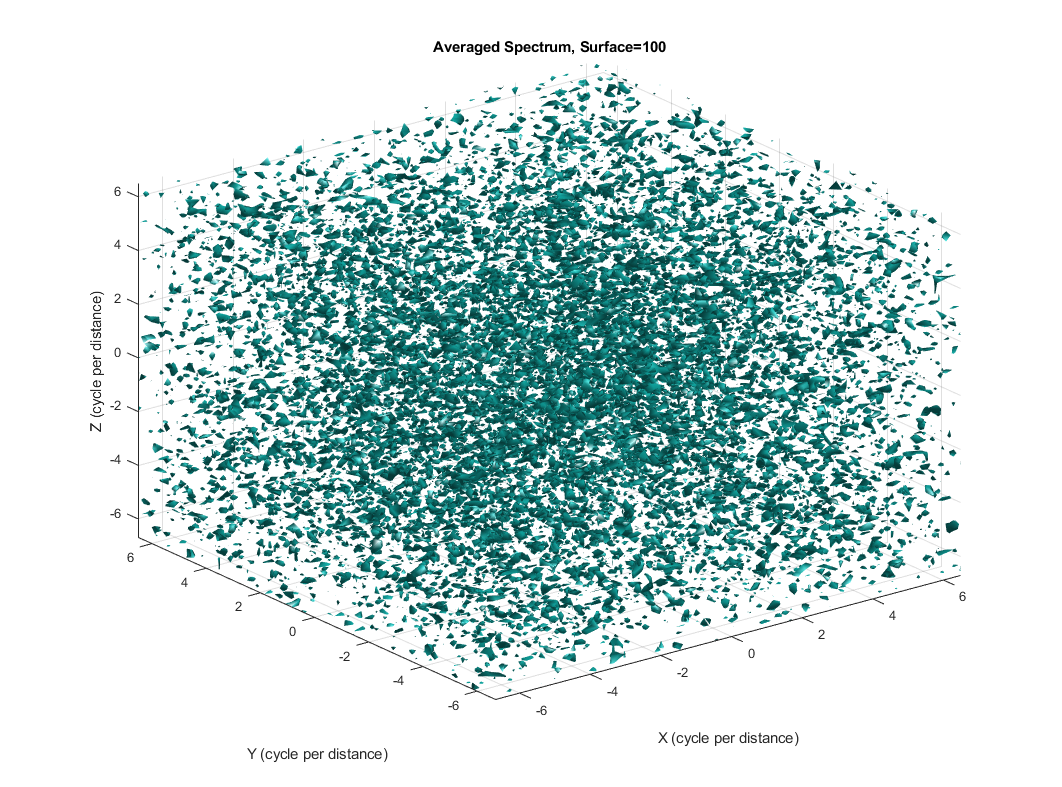
\includegraphics[width=\columnwidth]{avg_spectrum_thresh100.png}}
	\caption{Averaged spectrum, Threshold=100}\label{spect100}
\end{figure}


\begin{figure}
	\centerline{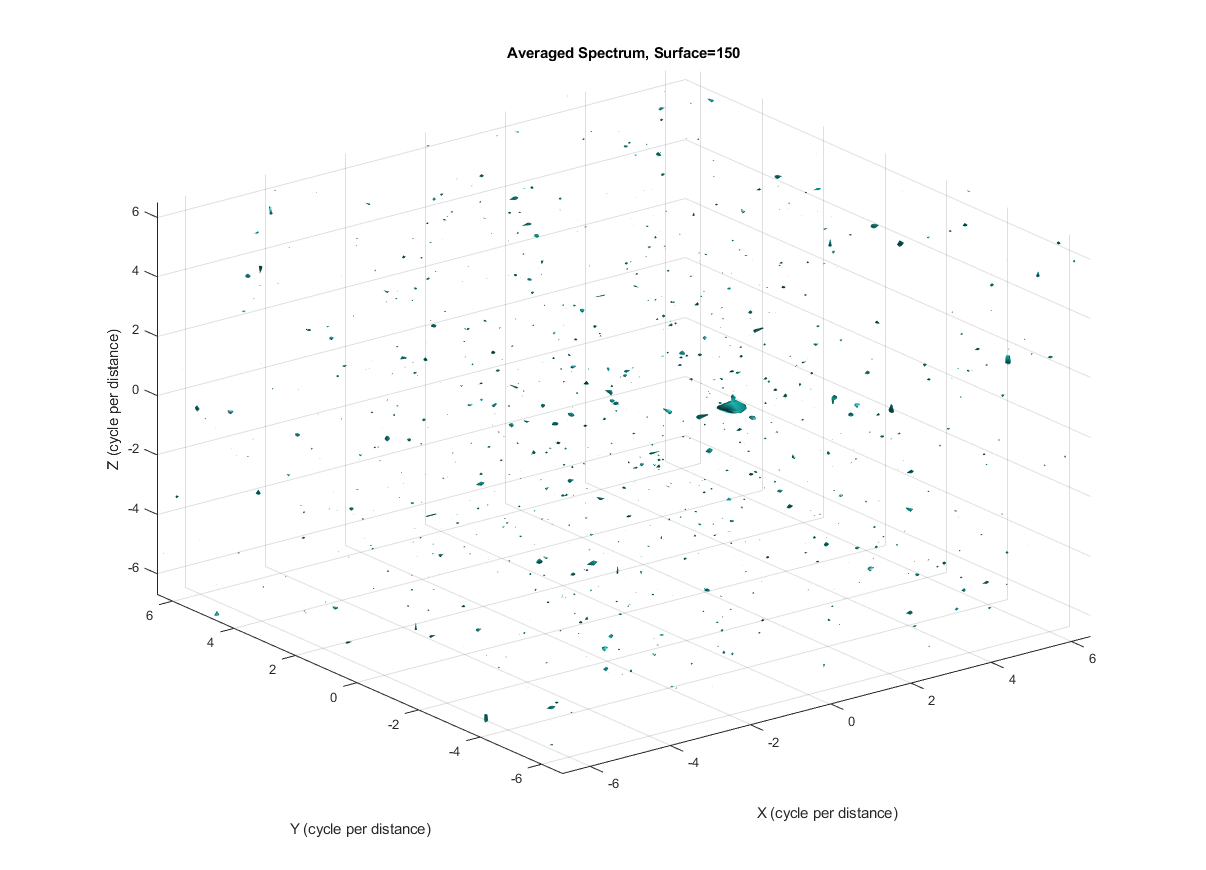
\includegraphics[width=\columnwidth]{avg_spectrum_thresh150.png}}
	\caption{Averaged spectrum, Threshold=150}\label{spect150}
\end{figure}


\begin{figure}
	\centerline{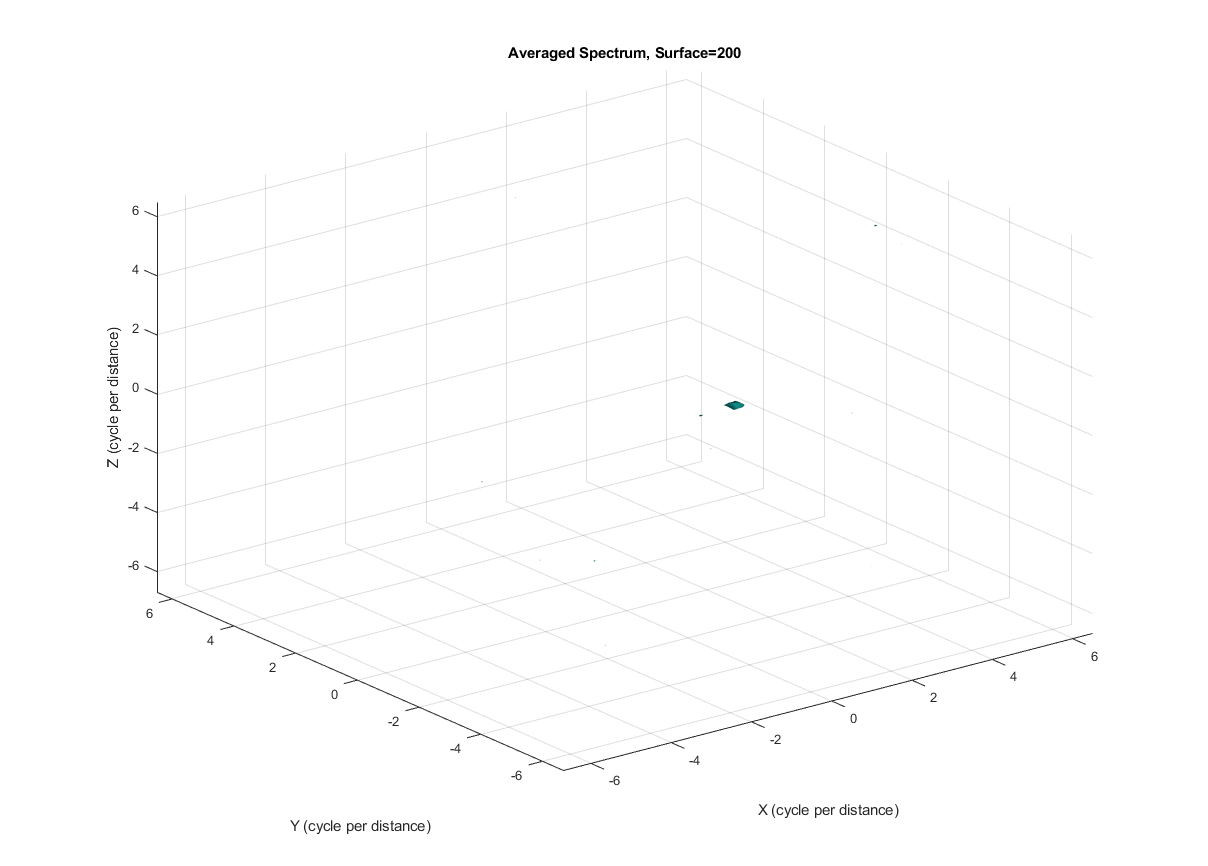
\includegraphics[width=\columnwidth]{avg_spectrum_thresh200.png}}
	\caption{Averaged spectrum, Threshold=200}\label{spect200}
\end{figure}


Using the most stringent \code{isosurface} threshold, the plot was manually inspected to determine the location of the maxima of the whole spectrum. These values were used to set the guassian kernel offsets. The kernels standard deviation was selected somewhat arbitrarily as 1, but the results appeared satisfactory. An improvement for a production environment would involve determining the maximum location in the spectrum programatically, but for exploratory work this was deemed acceptable in the interim.

To apply the filter (Fig. \ref{kernel_isosurface}), each spectrum was \code{fftshift}-ed and multiplied by the filter kernel, a process commonly known as convolution. This process could likely be optimized to be more performant if the volume of data was larger or there were specific latency requirements, but no preemptive attempts were made. The results were then again \code{fftshift}-ed and an inverse FFT was taken via \code{ifftn} to bring each filtered spectrum into the spatial domain.

\begin{figure}
	\centerline{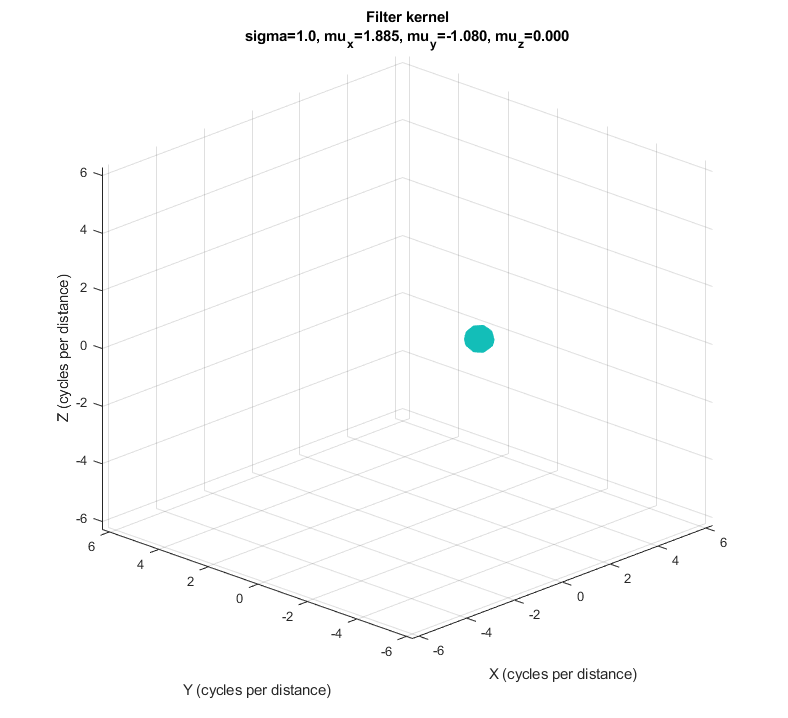
\includegraphics[width=\columnwidth]{filter_isosurface.png}}
	\caption{Normalized Gaussian Filter Kernel, threshold=0.9/1.0}\label{kernel_isosurface}
\end{figure}


Within each loop, another histogram was taken and plotted (Fig. \ref{filt_hists}) to determine verify the proper application of the filter and to determine an appropriate cutoff for \code{isosurface} plots.

\begin{figure}
	\centerline{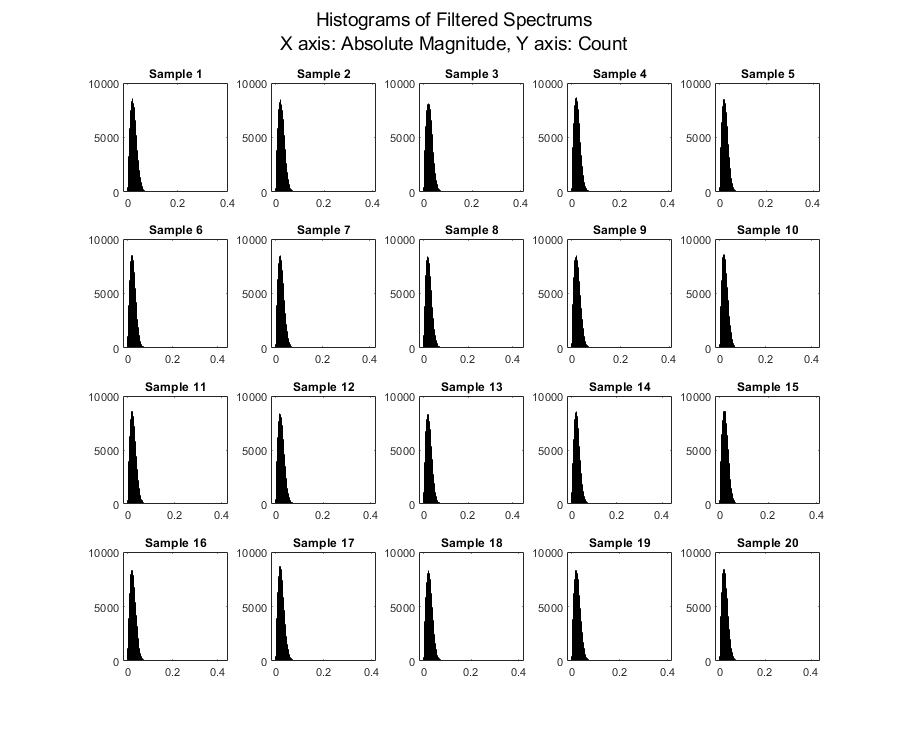
\includegraphics[width=\columnwidth]{filtered_spectrum_hists.png}}
	\caption{Filtered Spectrum Histograms}\label{filt_hists}
\end{figure}


Initially, each \code{isosurface} was plotted separately, but this was converted to plot each on the same figure in order to show the trajectory of the marble (Fig. \ref{traj_iso}). To indicate the temporal trend of each sample, each isosurface was shaded differently, going from light to dark in time. Note that in the code, due to differences in indexing between \code{meshgrid} and \code{ind2sub}, the X and Y mesh axes have been swapped to match the \code{plot3} trajectory.

\begin{figure}
	\centerline{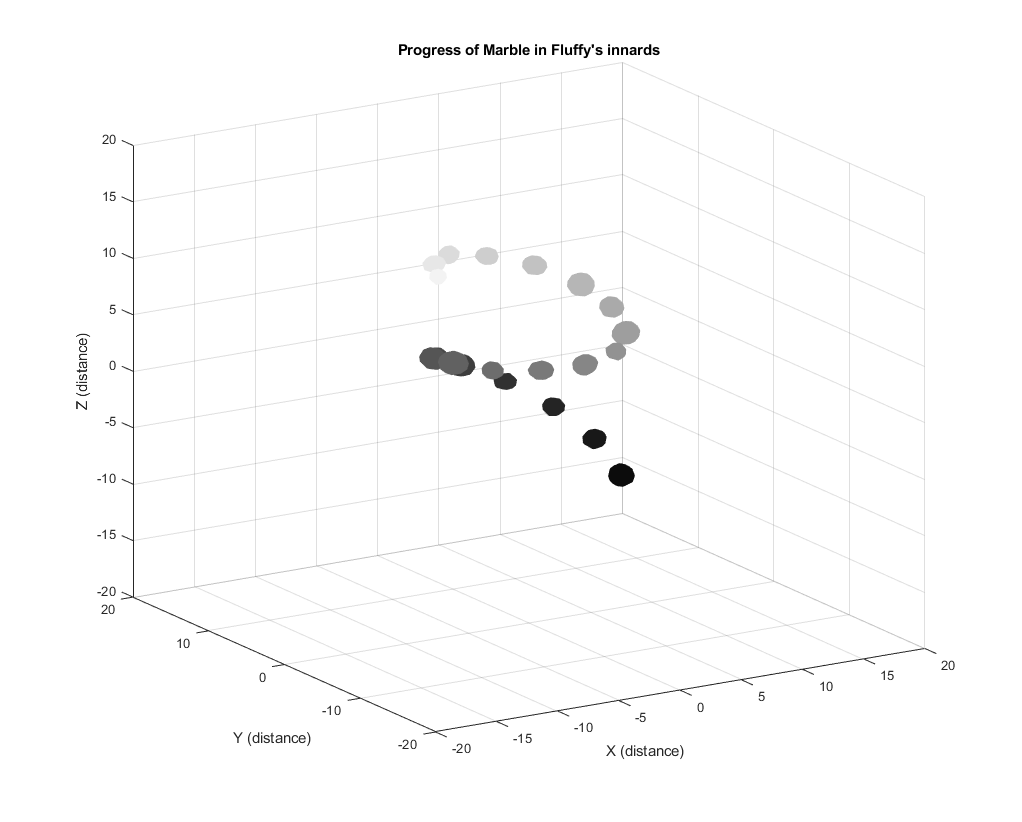
\includegraphics[width=\columnwidth]{trajectory_isosurface.png}}
	\caption{Trajectory of the marble as an isosurface}\label{traj_iso}
\end{figure}


Finally, per the requirements of the assignment, the peak of each filtered spatial sample was used to plot the trajectory with \code{plot3}, along with careful scaling of the indices (determined via \code{max} and \code{ind2sub}) to reflect the spatial domain (Fig. \ref{traj_max}).

\begin{figure}
	\centerline{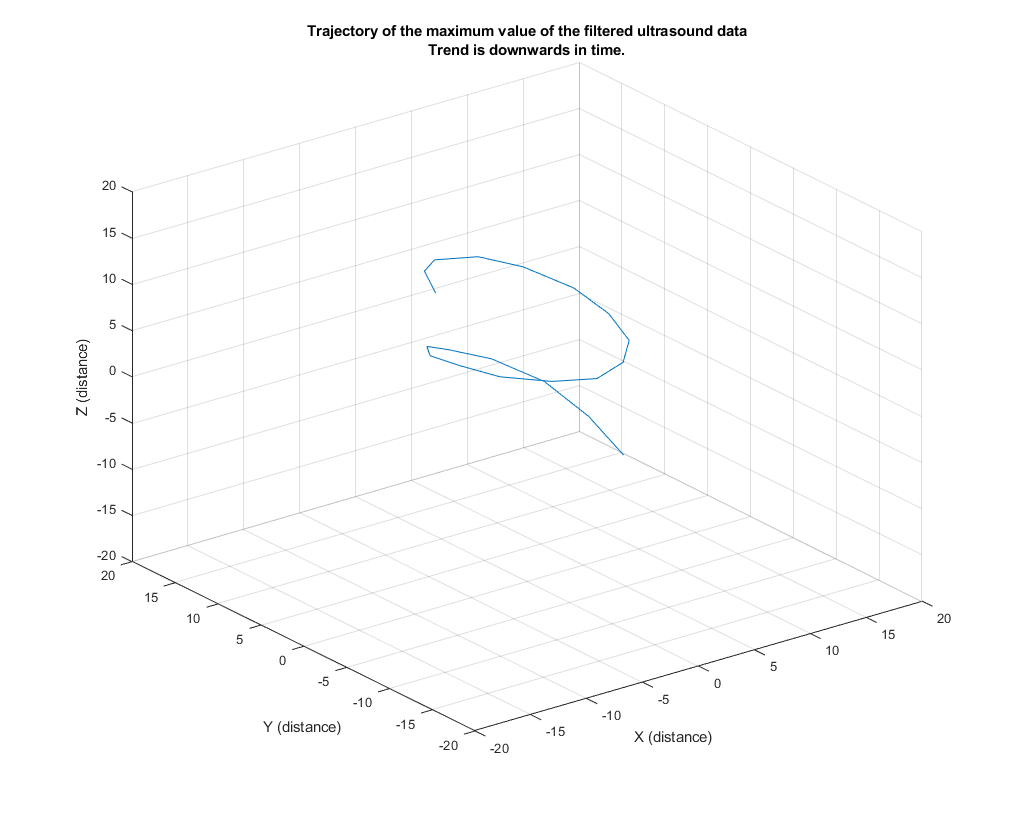
\includegraphics[width=\columnwidth]{trajectory_max_plot3.png}}
	\caption{Trajectory as determined by the maximum value of the filtered data}\label{traj_max} 
\end{figure}

\section{Computational Results}

The center frequency of the filter was determined to be at:

\begin{equation}
\omega_x=1.885
\end{equation}
\begin{equation}
\omega_y=-1.08
\end{equation}
\begin{equation}
\omega_z=0.0
\end{equation}
\noindent cycles per unit distance.

Based upon this trajectory, the vet should direct a blast of energy at:
\begin{equation}
x=4.688
\end{equation}
\begin{equation}
y=-5.156
\end{equation}
\begin{equation}
z=-5.625
\end{equation}

\noindent units of distance.

\section{Summary and Conclusion}
By taking advantage of the stochastic, stationary nature of noise and the power of the Fourier transform, one can resolve even highly noisy data into meaningful trends. At least, Fluffy appreciates it.

\newpage
\clearpage
\newpage
\section{Appendix A: Functions Used}
\subsection{\code{abs}}
Given a scalar, vector, or N dimensional matrix, returns a structure of the same size with all elements set to the absolute value of the original structure. Produces all positive numbers when the input is purely real, and produces purely real numbers when the input is complex.
\subsection{\code{fftn, ifftn}}
The n-dimensional fast Fourier transform (and its inverse). The prior assumes data is non-shifted, whereas the latter assumes it has been. The prior returns shifted data, the latter returns unshifted.
\subsection{\code{fftshift, ifftshift}}
Because \code{fft} and \code{fftn} produce data that has been shifted, \code{fftshift} is provided to undo the operation. Similarly, because \code{ifft} and \code{ifftn} expect the data to be shifted, \code{ifftshift} was provided to re-shift the data in preparation. In 1D, the data is swapped about the midpoint; in 2D, the quadrants are swapped diagonally, and so on into higher dimensions.
\subsection{\code{meshgrid}}
When given a pair of vectors containing cooordinates, returns a 2D grid coordinates for plotting 3D images (such as surface plots). When given 3 vectors, returns 3D grid coordinates for 4D plots (such as isosurface).
\subsection{\code{isosurface}}
Given a 3D mesh grid coordinates, a 3D matrix of magnitudes at each point defined in the grid coordinates, and a threshold value, produces a plot showing the surface(s) that connects all points equal to the threshold within the 3D space. If no threshold is provided, it determines one automatically. Analogous to a contour map, but in higher dimensions.
\subsection{\code{histogram}}
Given a vector or N-dimensional matrix, plots the distribution of the data after sorting it into bins. That is, provides a bar chart of the count of each number of elements that fit within a range (or "bin").
\subsection{\code{sprintf}}
Provides a C-like function for string formatting. Useful for programattically defining plot titles or messages to display.
\subsection{\code{disp}}
Displays its arguments to the command line. Useful for printing messages and variable values, preferred to eschewing semicolon suppression.
\subsection{\code{patch}}
Creates a graphics object composed of one or more polygons. Used for displaying more advanced plots or arbitrary shapes/objects.
\subsection{\code{isonormals}}
Similar to \code{isosurface}, but accepts a \code{patch} object and gives greater control over the appearance of the resulting plot.
\subsection{\code{max}}
Given a vector, returns the largest value and its location. For higher dimensional data, returns a subspace containing the highest value as a vector. Often most easily used when flattening a higher dimensional structure and using in conjunction with \code{ind2sub}.
\subsection{\code{ind2sub}}
Given a linear index and the shape of a data structure, converts from a linear index to the N-dimensional indices.
\subsection{\code{plot3}}
Given 3 vectors of positions in time (x, y, and z), produce a 3D plot of the path.
\subsection{Plotting Functions}
Functions, such as \code{figure}, \code{axis}, \code{subplot}, etc., are deemed trivially understood/searched for and thus not explained here.

\end{document}
